\documentclass[a11paper, 10pt]{article}
\usepackage[english]{babel}
\usepackage[utf8]{inputenc}
\usepackage{float}
\usepackage{verbatim}
\usepackage{listings}
\usepackage{graphicx}
\usepackage{a4wide}
\usepackage{color}
\usepackage{enumitem}
\usepackage{amsmath}
\usepackage{amssymb}
\usepackage[dvips]{epsfig}
\usepackage[T1]{fontenc}
\usepackage{cite} % [2,3,4] --> [2--4]
\usepackage{shadow}
\usepackage{hyperref}
\usepackage{cleveref}
\usepackage{siunitx}
\usepackage{caption}
\usepackage{subcaption}
\usepackage{multicol}
\usepackage{cancel}

\setcounter{tocdepth}{2}
\newcommand{\rmd}{{\mathrm d}}

\newcommand{\oder}[2]{\frac{{\rm d}#1}{{\rm d}#2}}
\newcommand{\odder}[2]{\frac{{\rm d}#1}{{\rm d}#2}}
\newcommand{\pd}[1]{\frac{\partial}{\partial #1}}
\newcommand{\pdt}[2]{\frac{\partial #1}{\partial #2}}
\newcommand{\pddt}[2]{\frac{\partial^2 #1}{\partial #2^2}}
\newcommand{\tpddt}[2]{\tfrac{\partial^2 #1}{\partial #2^2}}
\newcommand{\pdtfix}[3]{\frac{\partial #1}{\partial #2}_#3}

\newcommand{\npdt}[3]{\frac{\partial^{#3} #1}{\partial #2^{#3}}}

\newcommand{\angstrom}{\mbox{\normalfont\AA}}

\lstset{language=python}
\lstset{basicstyle=\small}
\lstset{backgroundcolor=\color{white}}
\lstset{frame=single}
\lstset{stringstyle=\ttfamily}
\lstset{keywordstyle=\color{red}\bfseries}
\lstset{commentstyle=\itshape\color{blue}}
\lstset{showspaces=false}
\lstset{showstringspaces=false}
\lstset{showtabs=false}
\lstset{breaklines}


\title{MAT4110 - oblig 1} 
\author{Halvard Sutterud }
\date{September 2018}

\begin{document}

\maketitle

\section{Theory and methods}
\subsection*{Exercise 1}
The QR-factorization decomposes a $n\times m$ matrix $A$ (with $n \geq m$)by

\begin{equation}
    A = QR,
\end{equation}

where $Q \in \mathbb{R}^{n \times n}$ is orthogonal and $R \in \mathbb{R}^{n\times m}$
is a matrix 

\begin{equation}
    R = \begin{pmatrix}
        R_1 \\ 0
    \end{pmatrix},
\end{equation}

where $R_1 \in \mathbb{}$ is upper triangular. The linear problem can then
be written as 

\begin{equation}
    Ax = b \Rightarrow Rx = Q^{-1}b = Q^Tb
\end{equation}

since $Q$ is orthogonal. As $R$ has $n-m$ rows consisting of zeros, these
will not contribute, and we simplify the problem further

\begin{equation} \label{eq:upper_triag}
    R_1 x =  c_1.% Q_1^T b,
\end{equation}

Here $c_1$ comes from the decomposition $Q^Tb = [c_1, c_2]$, where $c_1$
has length $m$ and $c_2$ has length $n-m$. As $R_1$ is upper triangular, we
can solve \cref{eq:upper_triag} by simple backwards substitution, 

\begin{align*}
    x_m &= \frac{c_m}{R_{m,m}}\\
    x_i &= \frac{c_i - \sum_{j=i+1}^{m} R_{i,j} x_j}{R_{i,i}} \quad \text{for}\quad i <
    m.
\end{align*}

This is implemented for our design matrix $X$ in the function \texttt{ex1}
in the python code, as can be seen in listing~\ref{lst:oblig1}. 

\subsection*{Exercise 2}
The cholesky factorization is a factorization of a symmetric $n\times n$
matrix $A = LDL^T$, where $L$ is lower triangular, and $D$ is diagonal. In the case that $A$ is positive definite (which it
is in our case, as $A = X^TX$), this can be rewritten 

\begin{equation}
    A = RR^T,
\end{equation}

if one writes $R = L D^{1/2}$, with $D^{1/2}$ as a matrix with the square
root of the diagonal elements of $D$ along the diagonal, i.e.
$(D^{1/2})_{i,i}  = \sqrt{D_{i,i}}$. 

The problem we wish to solve is 

\begin{equation}
    X^T X x = X^T b \Rightarrow Ax = X^T b
\end{equation}

We rewrite the problem by
performing the cholesky factorization on the symmetric matrix $A$,
%
\begin{equation}
     RR^Tx = X^T b,
\end{equation}
%
and then splitting this into a forward substitution 
%
\begin{equation}
     R y = X^T b,
\end{equation}
%
since $R$ is lower triangular, and a backward substitutiono
%
\begin{equation}
     R^T x = y,
\end{equation}
%
as $R^T$ is upper triangular.  This is implemented in the function
\texttt{ex2} in the python code, as can be seen in
listing~\ref{lst:oblig1}.  

\subsection*{Exercise 3}


The condition number when solving a linear system $Ax = b$ is given in the lecture
notes as the ratio of the largest singular value and the smallest,

\begin{equation}
    K_2(A) = \frac{\sigma_{\text{max}}
    (A)}{\sigma_{\text{min}}(A)}
\end{equation}

where $K_2$ indicates that we are using the 2-norm. In the QR-algorithm,
we solve the matrix equation $R_1x = c_1$, with $c_1 = Q_1 b$, and $R_1$
and $Q_1$ as the so-called economic matrices of the QR-factorization (as
provided by numpy). Applying the SVD-tranformation and calculating the K2-conditioning, we
get $K_2(R_1) = 58.95$ (for the given seed).

In the case of the cholesky solver, the problem solved is 

\begin{equation}
    RR^T x = A^T b
\end{equation}.

We solve it by two separate problems, $R^T x = y$ and $Ry = A^Tb$. However,
it can be shown that (left as an exercise to the reader)

\begin{equation}\label{eq:chol}
    K_2(RR^T) = K_2(R) K_2(R^T) = K_2(R)^2,
\end{equation}

which is good, because the conditioning should be independent of the way we
solve the problem (\cref{eq:chol}). Applying this to the given seed, we get
$K_2(R)^2 = (58.95)^2 = 3475.16$. We observe that the conditioning of the
original problem can be increased by increasing the number of times we
solve a linear system. 


\section{Results}

The resulting polynomials for the two functions stated in the problem set
can be seen in \cref{fig:data1,fig:data2}


\begin{figure}[htpb]
    \centering
    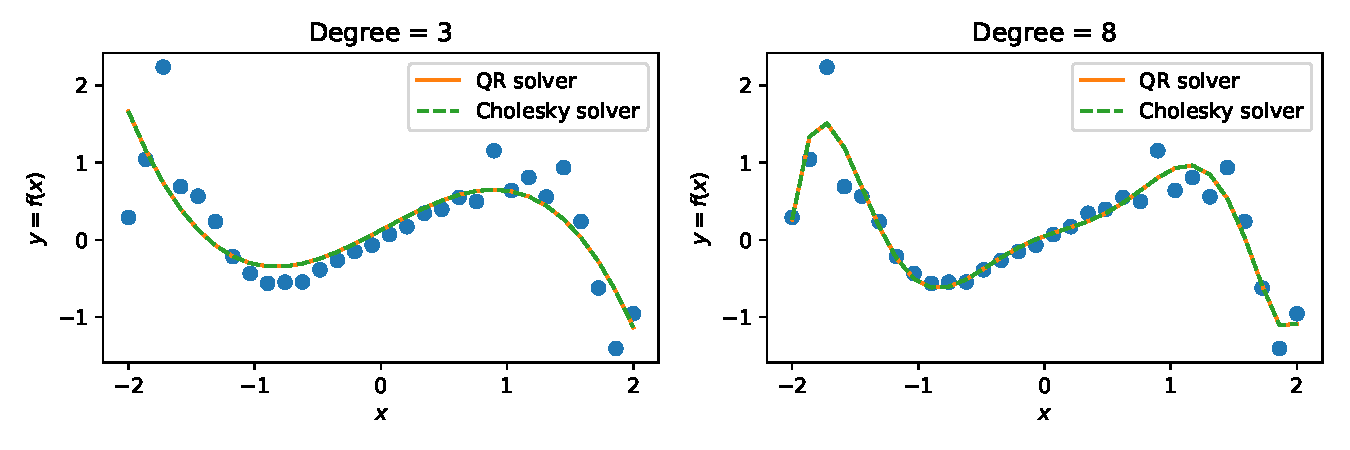
\includegraphics[width=0.8\linewidth]{data1.pdf}
    \caption{The first data as described in the problem set, fit with least
    squares solved by both $QR$-factorization and cholesky-factorization,
for polynomials of degree $3$ and $8$.}
    \label{fig:data1}
\end{figure}
\begin{figure}[htpb]
    \centering
    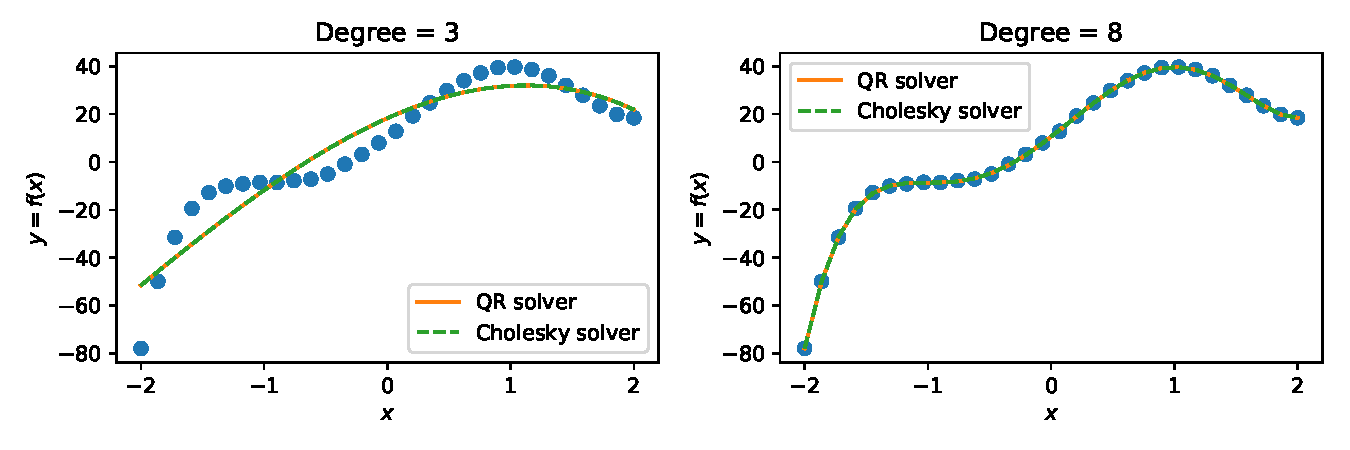
\includegraphics[width=0.8\linewidth]{data2.pdf}
    \caption{The second data as described in the problem set, fit with least
    squares solved by both $QR$-factorization and cholesky-factorization,
for polynomials of degree $3$ and $8$.}
    \label{fig:data2}
\end{figure}
\newpage

\lstinputlisting[label={lst:oblig1},caption={The file \texttt{oblig1.py}
}]{oblig1.py}

\end{document}
